\section{Mechanisms Behind the Effect of Health Insurance}
\label{sec:healthinsurance}

In the United States, healthcare is generally not provided directly by the government.
Instead, consumers purchase health insurance to fund healthcare expenses, with the government providing insurance only for elderly individuals (Medicare) and for those with low-incomes (Medicaid).
In 2004, the state of Oregon ceased accepting new applications for Medicaid due to budgetary constraints, and did not reopen applications until 2008.
When the state resumed enrolment, approximately 90,000 individuals applied, vastly exceeding the programme's capacity.
Oregon therefore allocated the opportunity to apply for Medicaid via a lottery system among those on the wait-list.
This wait-list lottery significantly increased health insurance coverage among the insurance applicants.

Winning the lottery increased health insurance coverage rate by 19 percentage points (pp).
This gave the opportunity to use the lottery as an instrument for having health insurance at all,\footnote{
    This additionally assumes everyone responded was at least more likely to take health insurance if they won the wait-list lottery, and the lottery did not have other direct effects.
} among the \input{../text/sections/tables/oregon-obs-count.txt} people from the wait-list lottery who responded to a survey sent by \cite{finkelstein2008oregon} one year later.
Among the wait-lottery compliers, having health insurance increased the rate of having visited the doctor (either locally or at a hospital) by 25 pp.
Furthermore, gaining insurance led to significant improvements in reported well-being: lottery compliers were 25 pp more likely to report being in good overall health, and 31 pp more likely to report being happy overall.
These statistics were calculated using the Oregon Health Insurance Experiment replication package \citep{icspr2014oregon}, and are summarised in \autoref{fig:healthinsurance-effects}.

\begin{figure}[!h]
    \caption{Effects of Health Insurance in the Oregon Health Insurance Experiment.}
    \centering
    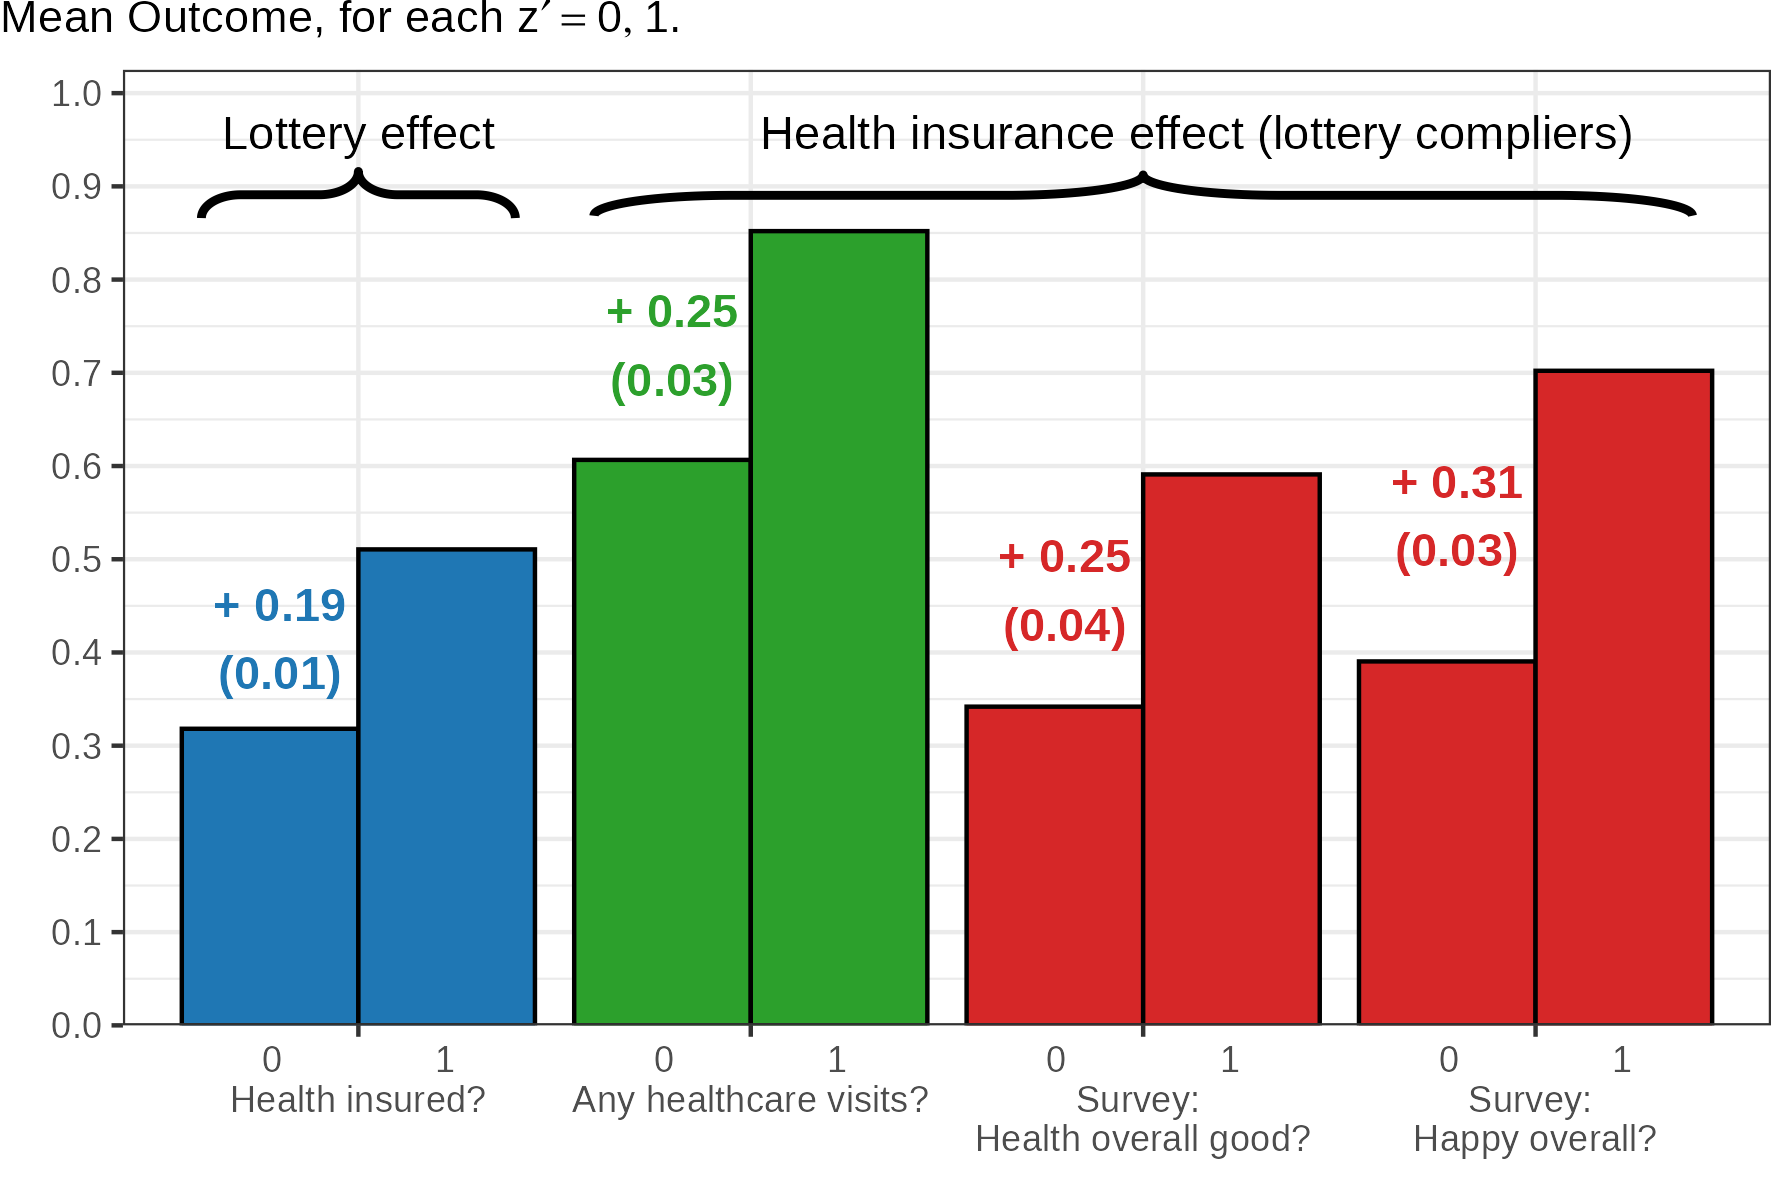
\includegraphics[width=0.85\textwidth]{sections/figures/insurance-effects.png}
    \label{fig:healthinsurance-effects}
    \justify
    \footnotesize    
    \textbf{Note:}
    This figure summarises the relevant results of the Oregon Health Insurance Experiment \citep{finkelstein2008oregon}.
    The lottery results show that winning the Medicaid wait-list lottery increased health insurance rate by 19 percentage points.
    The effect of health insurance shows estimates of the average lottery complier health insurance effect on surveyed outcomes.
    It uses the wait-list lottery as an instrument for having health insurance, and the \cite{abadie2003semiparametric} weighting scheme to estimate the average lottery complier levels, $\Egiven{Y_i(z',.)}{\text{lottery complier}}$ for each $z'=0,1$, with standard errors calculated by the bootstrap in brackets.
\end{figure}

These results show that health insurance led to large self-reported gains in both health and happiness.
The economics, medicine, and health policy literatures have primarily focused on the health benefits --- often interpreted as healthcare benefits among lottery compliers, who had previously delayed or avoided care due to cost concerns.
However, the original authors also noted other benefits of insurance, including complete elimination of catastrophic out-of-pocket medical debt among the treated.
% this was later followed up null results for the effect of health insurance on on clinically measured health outcomes \citep{baicker2013oregon}.
These are plausibly income effects that benefit recipients directly, not only through increased use of healthcare, but also by reducing stress and improving financial security.
These plausible direct effects have not been explored in the applied literature.

Accepted practice in applied economics is to investigate mechanisms behind treatment effects with ``suggestive evidence of mechanisms.''
This involves estimating the average causal effect of health insurance on a proposed mediator (healthcare usage) and separately estimating its effect on the final outcomes (self-reported health and happiness).
When both estimates are positive, and the mediator precedes the outcome, it is taken as de facto evidence that the mediator transmits the treatment effect.
In the case of the Oregon Health Insurance Experiment, this amounts to concluding that increased healthcare usage mediates the positive effects of health insurance on health and happiness.
\autoref{fig:scm-health} shows this approach in a stylised figure; the approach of suggestive evidence of mechanisms is also prevalent in other social sciences (see \citealt{blackwell2024assumption}).

\begin{figure}[!htbp]
    \centering
    \singlespacing
    \caption{Structural Causal Model for Suggestive Evidence of a Mechanism.}
    \label{fig:scm-health}
    \begin{tikzpicture}
        \node[state,thick,ForestGreen] (mediator) at (0,0) {$D_i$};
        \node[state,thick,blue] (treatment) [left=2.5cm of mediator] {$Z_i$};
        \node[state,thick,red] (outcome)   [right=2.5cm of mediator] {$Y_i$};
        % Label Z_i, D, Y_i
        \node[color=ForestGreen] [above=0.1cm of mediator] {Healthcare};
        \node[color=blue] [left=0.1cm of treatment] {Health insurance};
        \node[color=red] [right=0.1cm of outcome] {Health \& Happiness};
        % Draw the causal arrows
        \path[->, thick] (treatment) edge (mediator);
        %\path[->, dashed,color=gray] (mediator) edge (outcome);
        \path[->, thick] (treatment) edge[bend right=30] (outcome);
        % Label the IV.
        \node[state,thick,RoyalPurple] (treatmentIV) [above=0.75cm of treatment] {IV};
        \node[color=RoyalPurple] [left=0.1cm of treatmentIV] {Wait-list lottery};
        \path[->,thick,color=RoyalPurple] (treatmentIV) edge (treatment);
    \end{tikzpicture}
    \justify
    \footnotesize
    \textbf{Note}:
    This figure shows the structural causal model behind an inform mechanism analysis of the effects of health insurance, where arrows represent causal effects --- e.g., $Z_i \to D_i$ means $Z_i$ affects $D_i$ with no reverse causality.
    The variables correspond to the causal design in the Oregon Health Insurance Experiment.
\end{figure}

There are two main problems with this approach.
First, it provides no evidence for the effect of healthcare on health outcomes, so does not identify the causal mechanism.
It is hiding the assumption that healthcare positively affects health outcomes.
While this assumption is not unreasonable, nowhere else in applied economics is a hidden assumption of a positive treatment effect taken at face value --- it must be motivated with quantitative evidence.
Second, this approach does not quantify the mechanism effects.
The proportion of health insurance benefits operating through healthcare could only have small average effects in a 2 year span --- or possible very large, even dominant, if very strong.
Additionally, the relevant effect is not the average effect of healthcare usage, but the effect for Oregon residents who were induced to use more healthcare because of newly acquired Medicaid insurance. 
This local effect may differ substantially from a population average, and potentially mislead conclusions about the magnitude or generality of the mechanism.
To summarise, this approach is not suggestive evidence of mechanisms, it is assumptive evidence of mechanisms; it compels claims about mechanisms behind treatment effects which are not motivated by causal evidence.

% Paragraph here to describe the percent of papers that do this.
% As well as the number of papers who just blatantly control for the mediator, too.

Causal Mediation (CM) offers a compelling alternative framework.
Unlike suggestive evidence of mechanisms, CM explicitly defines the estimands of interest (the direct and indirect effects) and lays out clear assumptions under which these quantities are identified.
Moreover, it delivers quantitative answers to the key question: how much of a treatment effect operates through a specific mediator mechanism?
CM is widely used in fields such as epidemiology and psychology, where researchers regularly decompose treatment effects into component pathways.
However, CM methods have not yet been rigorously examined from an economic perspective to assess their applicability in observational causal research, such as natural experiments, which are the dominant source of identification in applied microeconomics.
